\documentclass[11pt]{article}

\usepackage{a4wide}
\usepackage{mathptm}
\usepackage{xspace}
\usepackage{amsmath}
\usepackage{graphicx}
\usepackage{algorithm}
\usepackage{algpseudocode}
\usepackage{tikz}
\usepackage{tkz-graph}
\usetikzlibrary{shapes.misc, positioning}
\usepackage{listings}
\usepackage{color}
\usepackage{minted}
\usepackage[utf8]{inputenc}
\usepackage{graphicx}
\usepackage[numbers,sort&compress]{natbib}
\usepackage[colorlinks,citecolor=red,urlcolor=blue,bookmarks=false,hypertexnames=true]{hyperref} 

\definecolor{codegreen}{rgb}{0,0.6,0}
\definecolor{codegray}{rgb}{0.5,0.5,0.5}
\definecolor{codepurple}{rgb}{0.58,0,0.82}
\definecolor{backcolour}{rgb}{0.95,0.95,0.92}
 
\lstdefinestyle{mystyle}{
    backgroundcolor=\color{backcolour},   
    commentstyle=\color{codegreen},
    keywordstyle=\color{magenta},
    numberstyle=\tiny\color{codegray},
    stringstyle=\color{codepurple},
    basicstyle=\footnotesize,
    breakatwhitespace=false,         
    breaklines=true,                 
    captionpos=b,                    
    keepspaces=true,                 
    numbers=left,                    
    numbersep=5pt,                  
    showspaces=false,                
    showstringspaces=false,
    showtabs=false,                  
    tabsize=2
}
 
\lstset{style=mystyle}


\definecolor{dkgreen}{rgb}{0,0.6,0}
\definecolor{gray}{rgb}{0.5,0.5,0.5}
\definecolor{mauve}{rgb}{0.58,0,0.82}

\lstset{frame=tb,
  language=Java,
  aboveskip=3mm,
  belowskip=3mm,
  showstringspaces=false,
  columns=flexible,
  basicstyle={\small\ttfamily},
  numbers=left,
  numberstyle=\tiny\color{gray},
  keywordstyle=\color{blue},
  commentstyle=\color{dkgreen},
  stringstyle=\color{mauve},
  breaklines=true,
  breakatwhitespace=true,
  tabsize=3
}
\setlength{\parindent}{0pt}



\begin{document}


\title{Software Technology Evaluation Project}

\author{Hans I. Botnen, Mikal Fuglestein, Joakim M. Grutle, Philip T. Hoang}

\maketitle

\begin{abstract}
    The task for this project is to evaluate a software technology and the goal is to gain more knowledge about the evaluated technology. By evaluating and understanding a software technology, we will find out how and why such a technology is used. The software technology to be evaluated for this project is Node.js. An entirely new prototype web application inspired by our previous project in the course were created with both frontend and backend written in JavaScript, the language used in Node.js. Even though the project report and evaluation is based on Node.js, some other technologies are used in the prototype to make it work. The prototype is connected to an external database and is running a server from Node.js. The report goes in details about the Node.js and the prototype,the development and testing of the prototype, as well as the evaluation of our results. The prototype can be found in the group's GitHub repository \cite{prototype:repo}, in the folder ArtJungle.
\end{abstract}
\clearpage
%input{commands}
\clearpage
\section{Introduction}
\label{sec:introduction}
 The reason for our interest in this Node.js is its supposed simplicity combined with its quality of being powerful. Our motivation is also based on the fact that Node.js is a popular technology used in many popular real world applications today. We have created a prototype web application to use as a good base for evaluating Node.js. We will be looking into how simple and powerful Node.js is, and also compare the technology and results of this prototype to the Java EE project.
\\\\
Node.js, created by Ryan Dahl, was first introduced in 2009 as a 
open-source, cross-platform JavaScript run-time environment, running on Linux and Mac OS X (Windows launch in 2011). Dahl was inspired to create Node.js after using file upload on an image hosting service called Flickr, where the browser could not see how much of the file had been uploaded and had to query the Web server. Dahl criticized the limitations of concurrent connections in Apache HTTP servers. He strongly desired a solution to this problem, thus creating Node.js. As we will see later in the report, Dahl solved this concurrent connection problem in a clever way by combining several other technologies like Google's V8 JavaScript engine, an event loop and a low level I/O API. \cite{wiki:nodejs}
\\\\
New web technologies surface now and then, and these technologies offer 
many different solutions to different problems. Many popular Websites like Netflix, PayPal, LinkedIn and many more are using Node.js as one of their main technologies, but what makes Node.js stand out from other technologies? In this project we have implemented an auction application based on our previous project in this course. Just like the previous project we are running a server directly from Node.js, and connect our application to a remote database. We have been basing our design of this application (mostly) on the design of the previous project, so the functionality is almost the same. We will try to show through our hands-on experience why Node.js is more preferable than many other web technologies today.
\\\\
The rest of the this report is organized as follows: 
\begin{itemize}
\item Section "Background": an overview about the software technology, its history, architecture and functionality. 

\item Section "Demonstrator Prototype": high-level view of the software technology in action, how we implemented the prototype and a presentation of the prototype.

\item Section "Test Environment and Experimental Results": describes the software in a test-bed environment and what experiments have been done.

\item Section "Conclusion": gives an overview over the conclusions about the software technology, the prototype and what results we have achieved in this project.
\end{itemize}
\clearpage
\section{Background}
\label{sec:background}
Node.js is a JavaScript run-time environment that executes code outside of a browser. Node.js is built on Google's V8 JavaScript engine where the V8 is written in C++ and used to compile JavaScript code directly to native machine code before executing it. 
The technology also allows the user to create Web servers and networking tools using JavaScript and a collection of 'modules' that are used to handle various core functionality. 
\cite{wiki:nodejs}.

\subsection{Package Manager: Node Package Module}
As mentioned, Node.js allows the user to use a collection of modules for different tasks. They are installed from Node Package Module which is one of the most powerful tools of Node.js. The modules are installed from the command "npm install modulename" and the modules are downloaded to folder "{node\_modules}". Node Package Module started as a way to download dependencies, but has quickly become an important tool for working with JavaScript. The idea of npm modules is to have a set of reusable components that is available through an easy installation via an online repository that can be found at the npm website. \cite{npm:webpage}
\\\\
Every Node.js project comes with an package.json file. This file is the core of the Node.js ecosystem and describes what modules are required for a project. It manages modules of a project and also scripts for generating builds and running tests \cite{npmjs:modules}. 
The package.json file has some important properties that must be initialized before one can start on the project such as name, version, scripts and dependencies. 
\begin{figure}[h!]
  \centering
  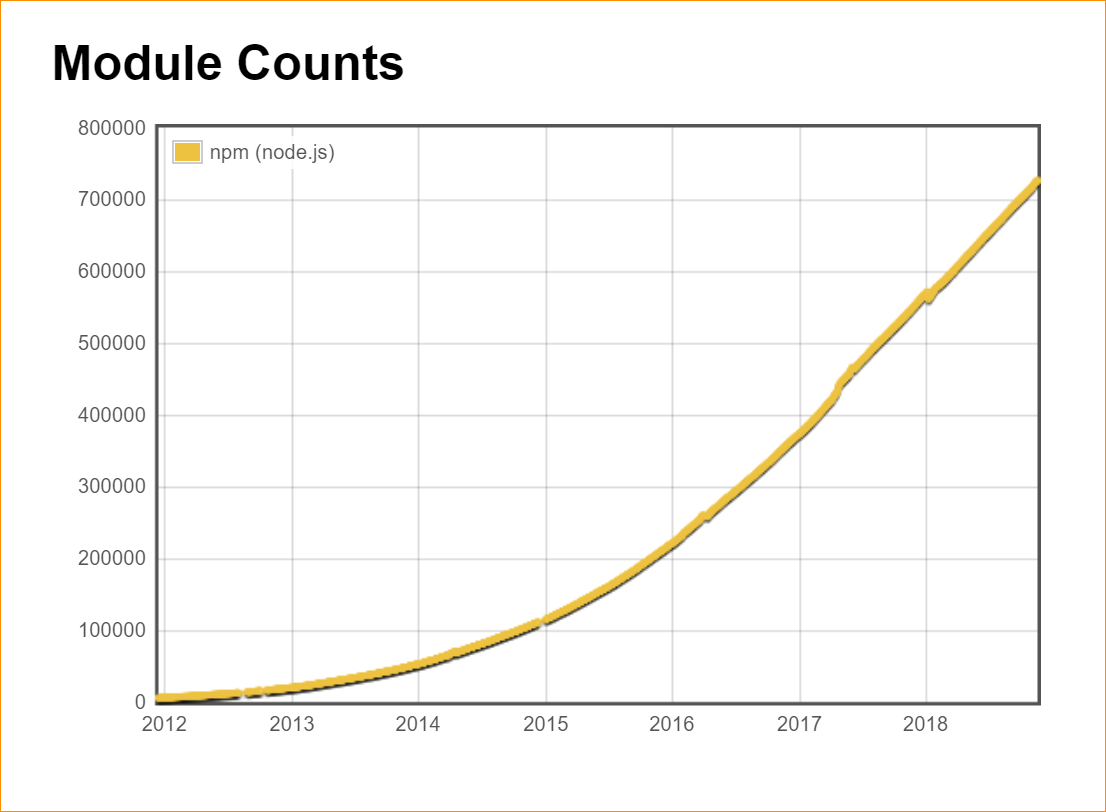
\includegraphics[scale=0.5]{figs/npmmodulescounts.png}
  \caption{How the number of modules have grown over the years \cite{image:modulecount}}
\end{figure}\\
One of the reasons why npm and Node.js became popular is because of how simple it is for developers to create new packages and how easy it is for others to use them. From figure 1 we can see that number of modules in npm has grown almost polynomial since its start. 
\\\\
Some of the most useful modules that we use in our prototype: 
\begin{itemize}
    \item Express: Web development framework (server) for Node.js and a standard for most Node.js applications.
    \item body-parser: A module that goes in hand with Express. Extracts the entire body of an incoming request stream from Express. Makes it easy to use JSON.
    \item Mongo/Mongoose: Wrappers to interact with MongoDB database in Node.js
    \item Socket.io: Real-time bidirectional event-based communication.  
\end{itemize}

\subsection{Single Thread and Event Loop}
Node.js uses 'Single Threaded Event Loop Model' architecture to handle multiple concurrent tasks versus other web application technologies like JSP, SPRING, HTML, etc., that follow 'Multi-Threaded Request-Response' architecture to handle multiple concurrent clients. 
\\\\
To compare, an example of a more traditional solution is a PHP application on an Apache server. Both Node.js and PHP can be used to to build network programs such as Web servers. The main difference between these technologies is that most functions in PHP block until termination, while functions in Node.js are non-blocking. This means that commands execute concurrently or even in parallel and use callbacks to signal completion (or failure). 
\\\\
Node.js works on a single thread because it uses non-block I/O calls. It allows the server to support multiple concurrent connections and the connections are held in an event loop, hence event-driven system.
It also optimizes throughout and scalability in web applications with many I/O operations, making Node.js applications extremely fast and efficient. \cite{docs:eventloop}

\begin{figure}[h!]
  \centering
  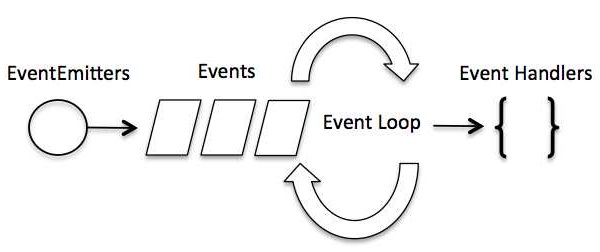
\includegraphics[scale=0.5]{figs/event_loop.jpg}
  \caption{Event Loop with an Event Emitter which listen to incoming events \cite{eventloop:image}}
\end{figure}

The design of using single thread event loop and sharing this thread among all the client is intended for building highly concurrent applications, where any function performing I/O must use a callback. A callback is a function that is to be executed after another function has finished executing \cite{codeburst:callback}. 
\\\\
Despite JavaScript being single-threaded, Node.js uses event loop to handle scalability instead of threads. With the event loop it is easier to handle multiple clients because there is no need to create more threads, and since Node.js uses less threads, it can utilize on less resources or memory. 
\\\\
When the Node.js server starts, the event loop get initialized and simply waits for events to occur. The event loop has an EventEmitter class that listens for events and triggers a callback function when an event is detected. 

\subsection{V8}
V8 engine is a open source JavaScript engine provided by Google. It is a engine that converts JavaScript code into lower level that microprocessors can understand. The V8 can run JavaScript standalone, but at we can also add our own function implementation to the engine.

\begin{figure}[h!]
  \centering
  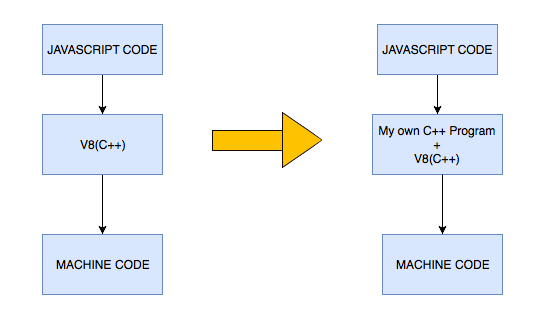
\includegraphics[scale=0.5]{figs/v8engine.png}
  \caption{Traditional Thread Solution vs. Node.js' Single Thread
  \cite{article:v8engine}}
\end{figure}

The V8 engine is written in C++ and Node.js in itself is a C++ implementation of the engine allowing server side programming and networking applications, and what Ryan Dahl did to achieve Node.js was that he added event I/O architecture, network- and HTTP-I/O libraries to the V8 engine. \cite{article:v8engine}

\subsection{Technology comparison to Java EE}
As we can see, Node.js is a well built technology, but how does it compare to the technology used in our previous project, Java EE? 
\\\\
Java EE uses standard Java as a language, which has a solid foundation and strong typing. Java EE applications often end up being very robust and resilient, much more so than an application created in JavaScript. But there are several reasons that JavaScript is one of the most popular languages in the world right now, one of the biggest reasons being it's simplicity compared to Java. Node.js utilizes this already simple language on both frontend and backend, resulting in a very simple development experience. 
\\\\
There is a lot of libraries and official documentation for Java EE, e.g., Oracle for documentation and Maven repository for libraries. The same goes for Node.js, which has the worlds biggest software registry at it's fingertips thanks to npm. Npm has become a very powerful tool for any JavaScript developer, even without Node.js. There is also a lot of official documentation for Node.js just like Java EE (though the Java EE documentation is much more mundane), but there is more relevant help to find online for Node.js (tutorials, forums, videos etc.), due to it's popularity.
\\\\
As mentioned earlier, Node.js creates a new single thread for handling concurrent function calls, whereas Java EE uses multithreading. Creating multiple threads may use extra time and memory, but it prevents complete blocking if a deadlock appears and it doesn't starve other threads if one is running slowly. It is worth noting that deadlocks are highly unlikely in Node.js because of non I/O blocking, which makes the technology more scalable, just like Java EE. \cite{compare:javanode} 
\\\\
As we have illustrated these two technologies have both similarities and differences. Both technologies are supposedly simple, powerful and versatile, but Java EE is also more robust. One is not necessarily better than the other and different applications have different needs, so the developer has to decide which language to use. Luckily we have been working with both technologies, and can hopefully give a good "in practice" comparison between the two when we examine our prototype. 
\section{Demonstrator Prototype}
\label{sec:prototype}

To construct a representative demonstrator prototype illustrating the use of Node.js, we developed a web application inspired from the Java EE project. By building the project from the bottom with Node.js using MongoDB and Express as tools, we developed a portal based on art commerce. The web application for auctioning artworks was constructed as a prototype to demonstrate the substantial assets and benefits of Node.js. Both back-end and front-end are implemented in JavaScript. 

\subsection{Prototype}
As mentioned, the prototype is inspired by the Java EE project with focus on artworks instead of products. Our main focus for this prototype (because of time constraints) was to implement the most essential features to make the application work as intended.
\\\\
The entities Artwork and Account are quite similar. Viewing accounts and arts in the application has the same layout. Creating an account and submitting an artwork are also similar with the exception of uploading an image when submitting an artwork, and therefore only showing images of functionalities for entity Artwork.

\begin{figure}[h!]
  \centering
  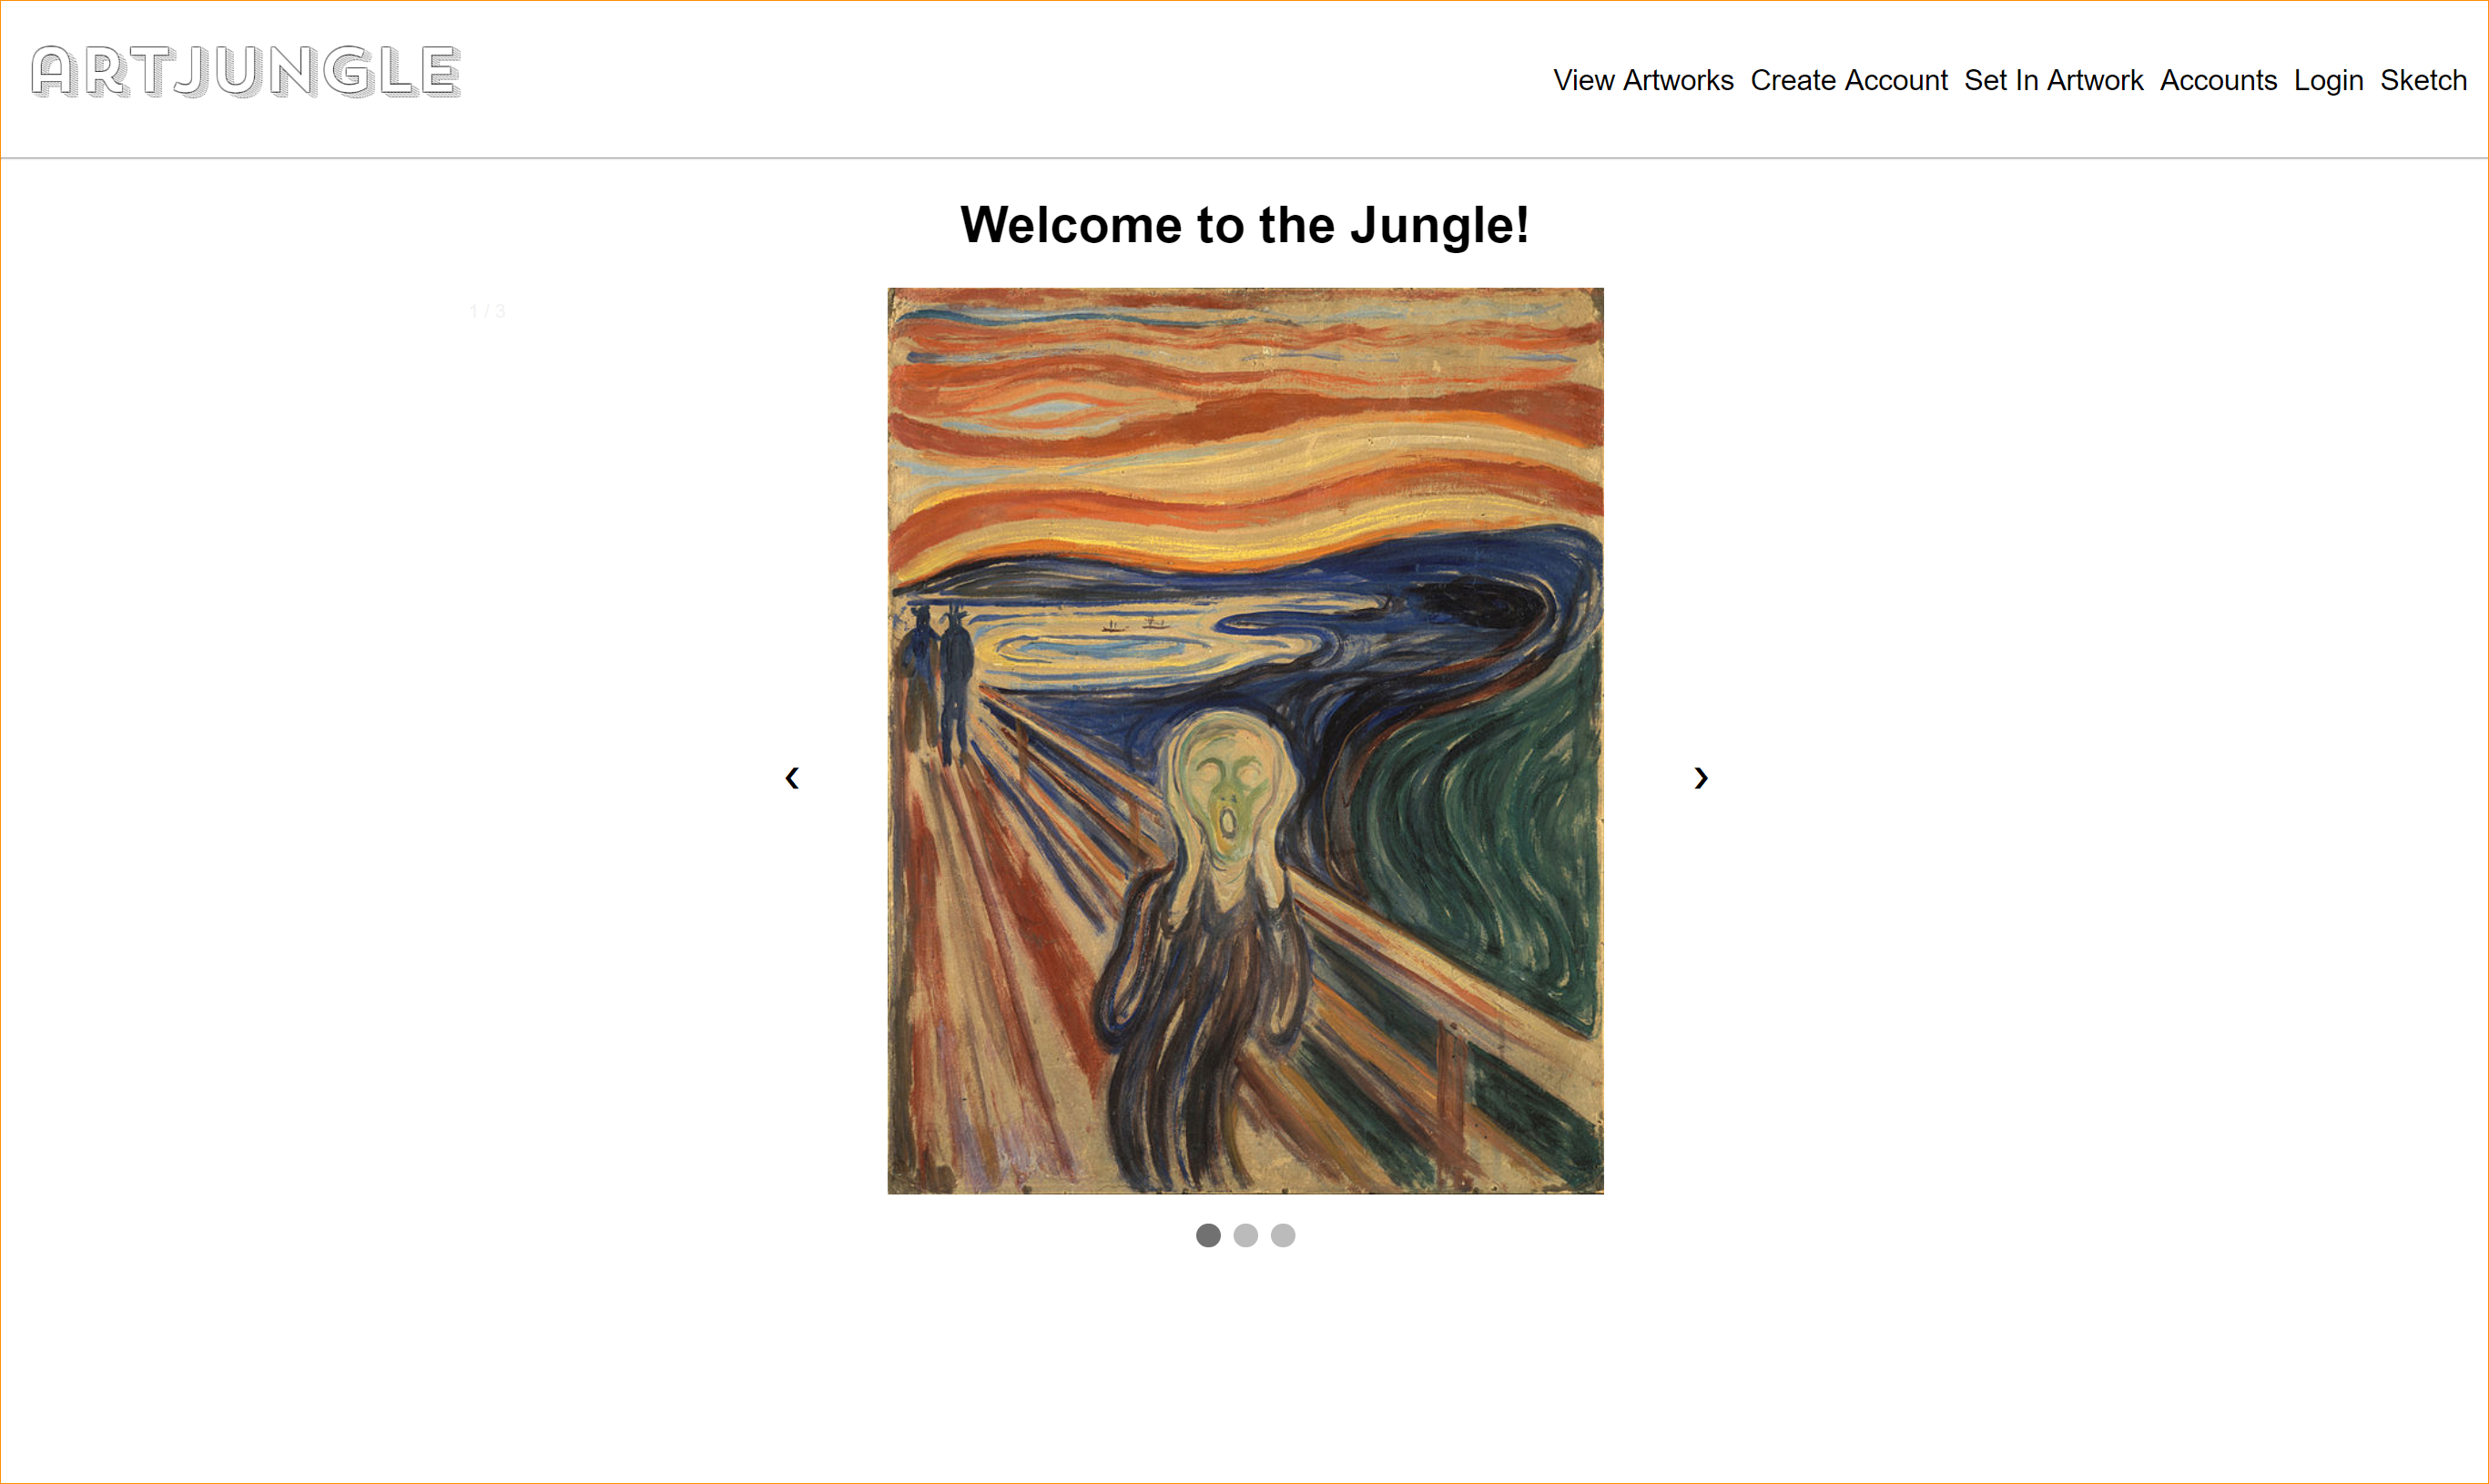
\includegraphics[scale=0.3]{figs/homescreen.png}
  \caption{Homescreen of the application}
\end{figure}

The home screen, as shown in figure 4, is very simple. The user will be met with a slideshow over some of the arts being available for auction. The user can also at any time navigate to other sites by clicking on a link in the header of the page. 

\begin{figure}[h!]
  \centering
  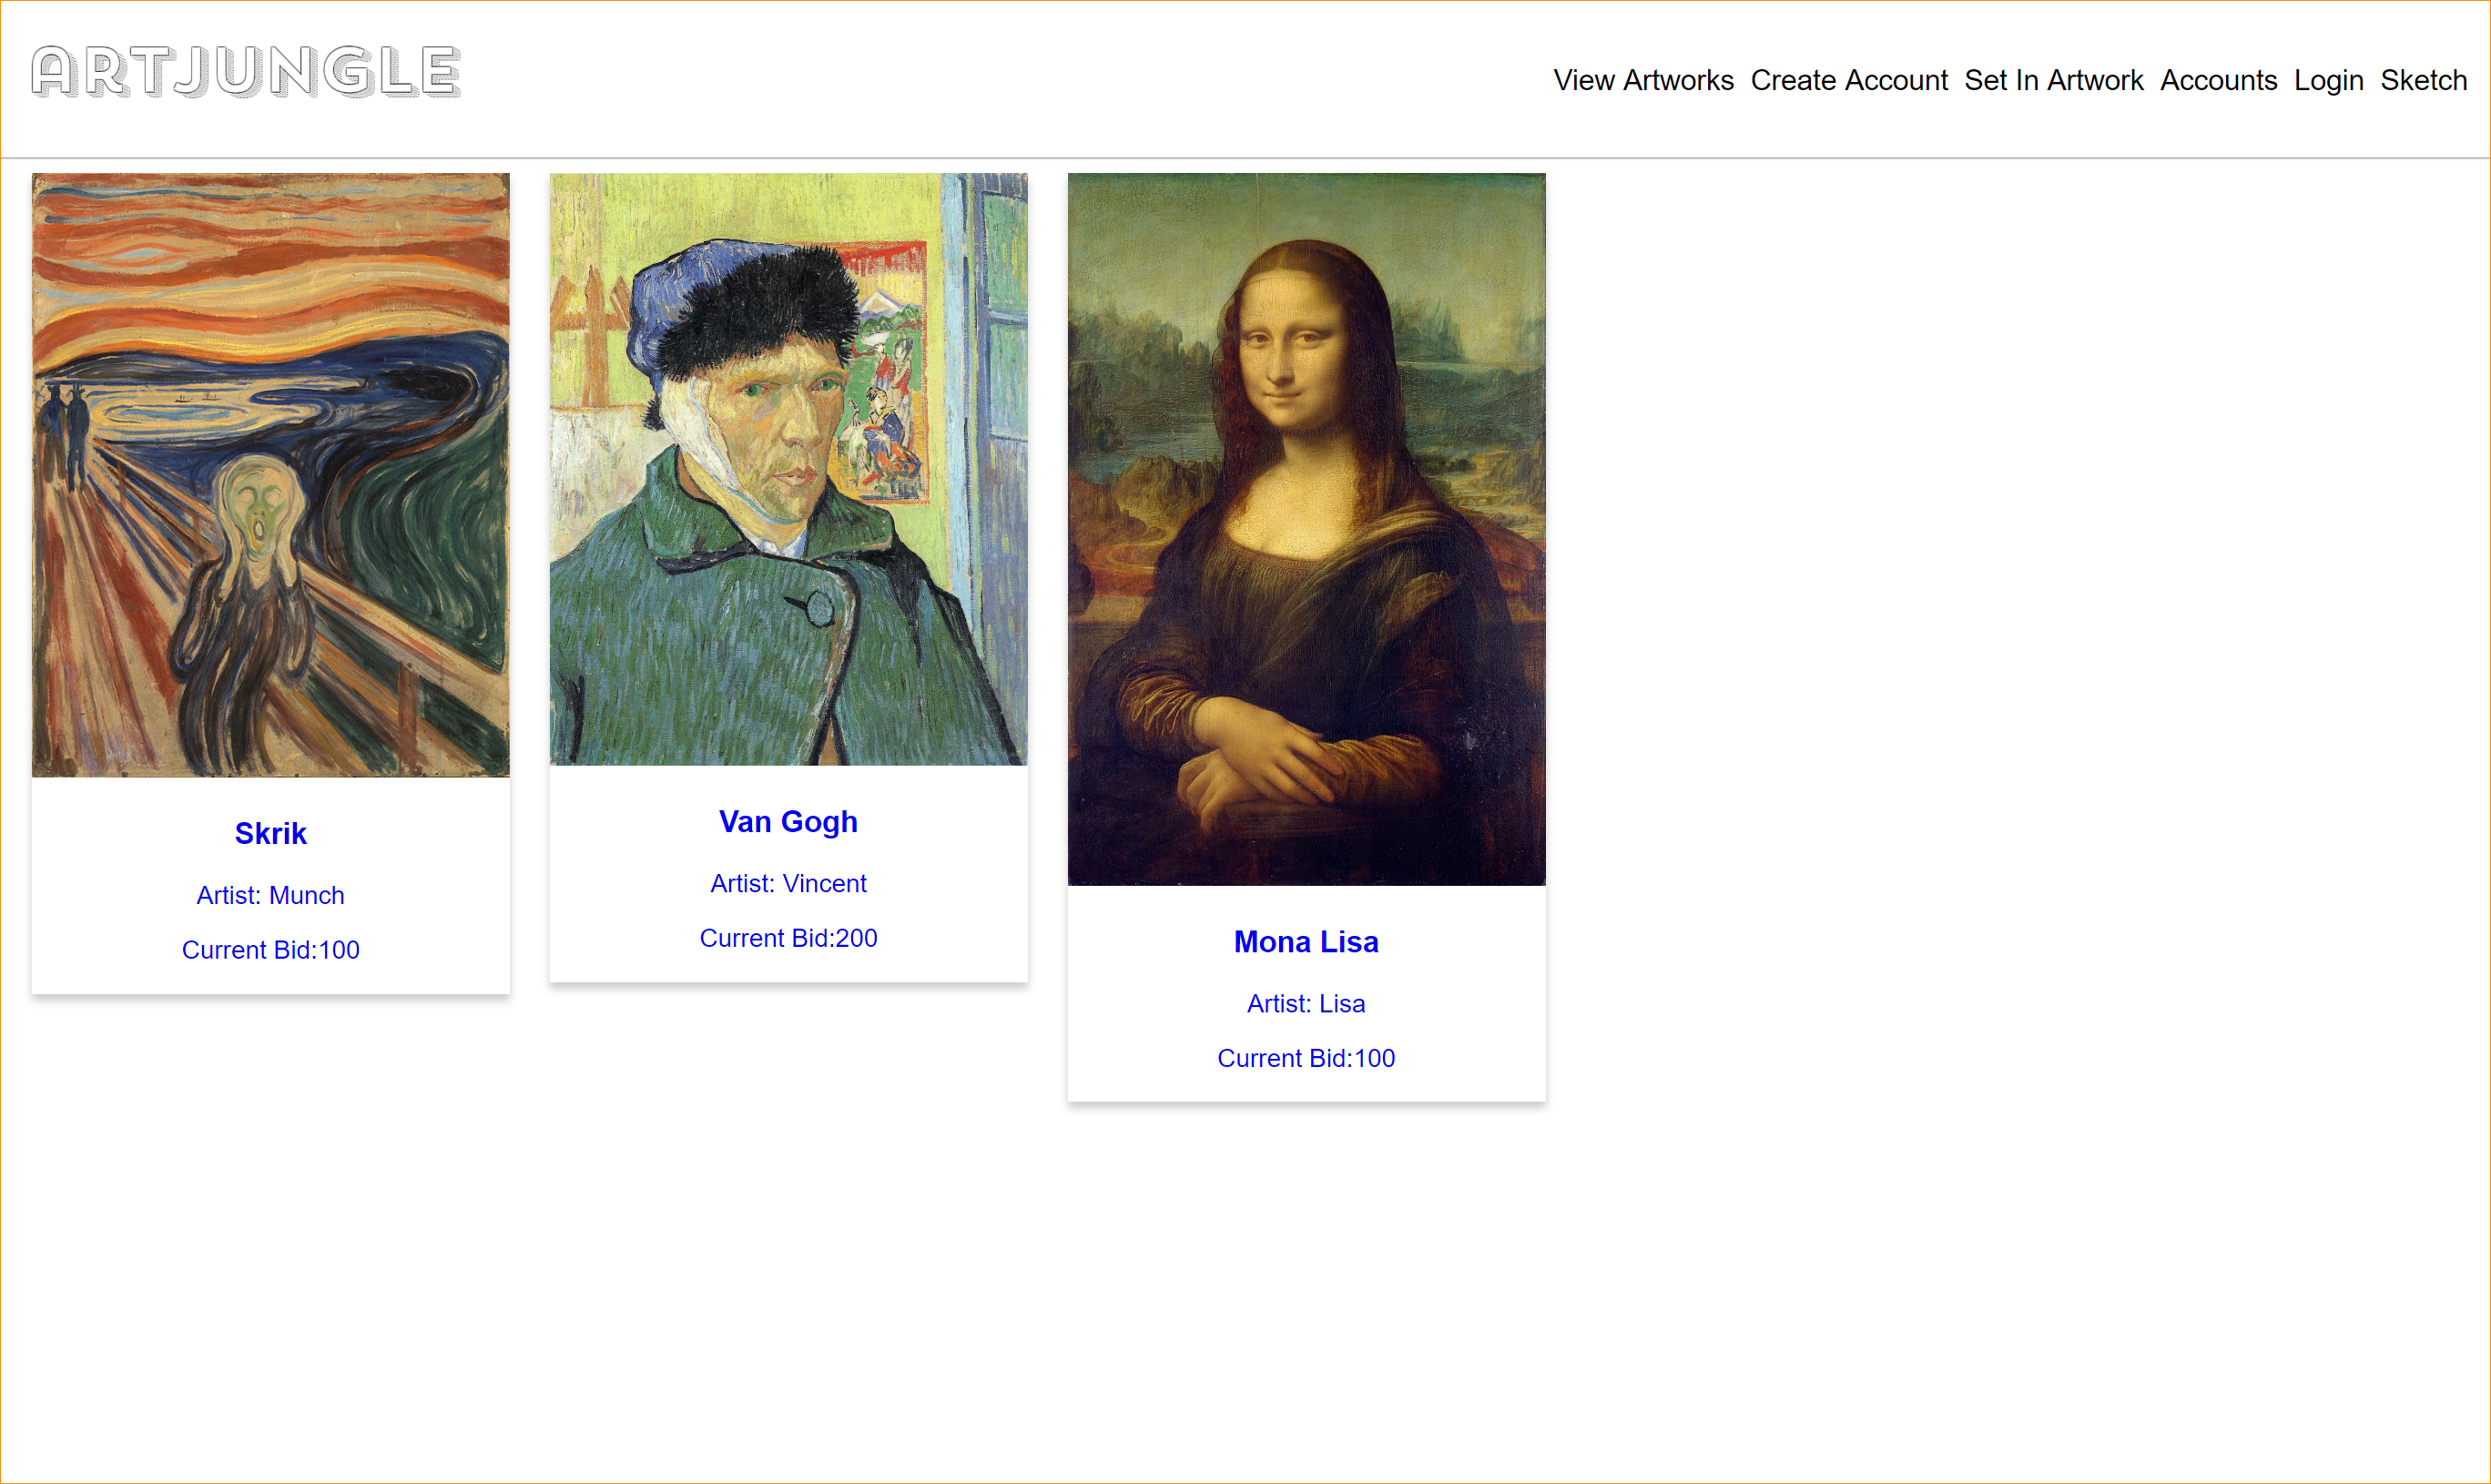
\includegraphics[scale=0.3]{figs/viewartworks.png}
  \caption{Overview of artworks}
\end{figure}

When navigating to "View Artworks", the user will see an overview of the artworks, as shown in figure 5. The user will be able to click on an artwork to get more details about that particular artwork. 

\begin{figure}[h!]
  \centering
  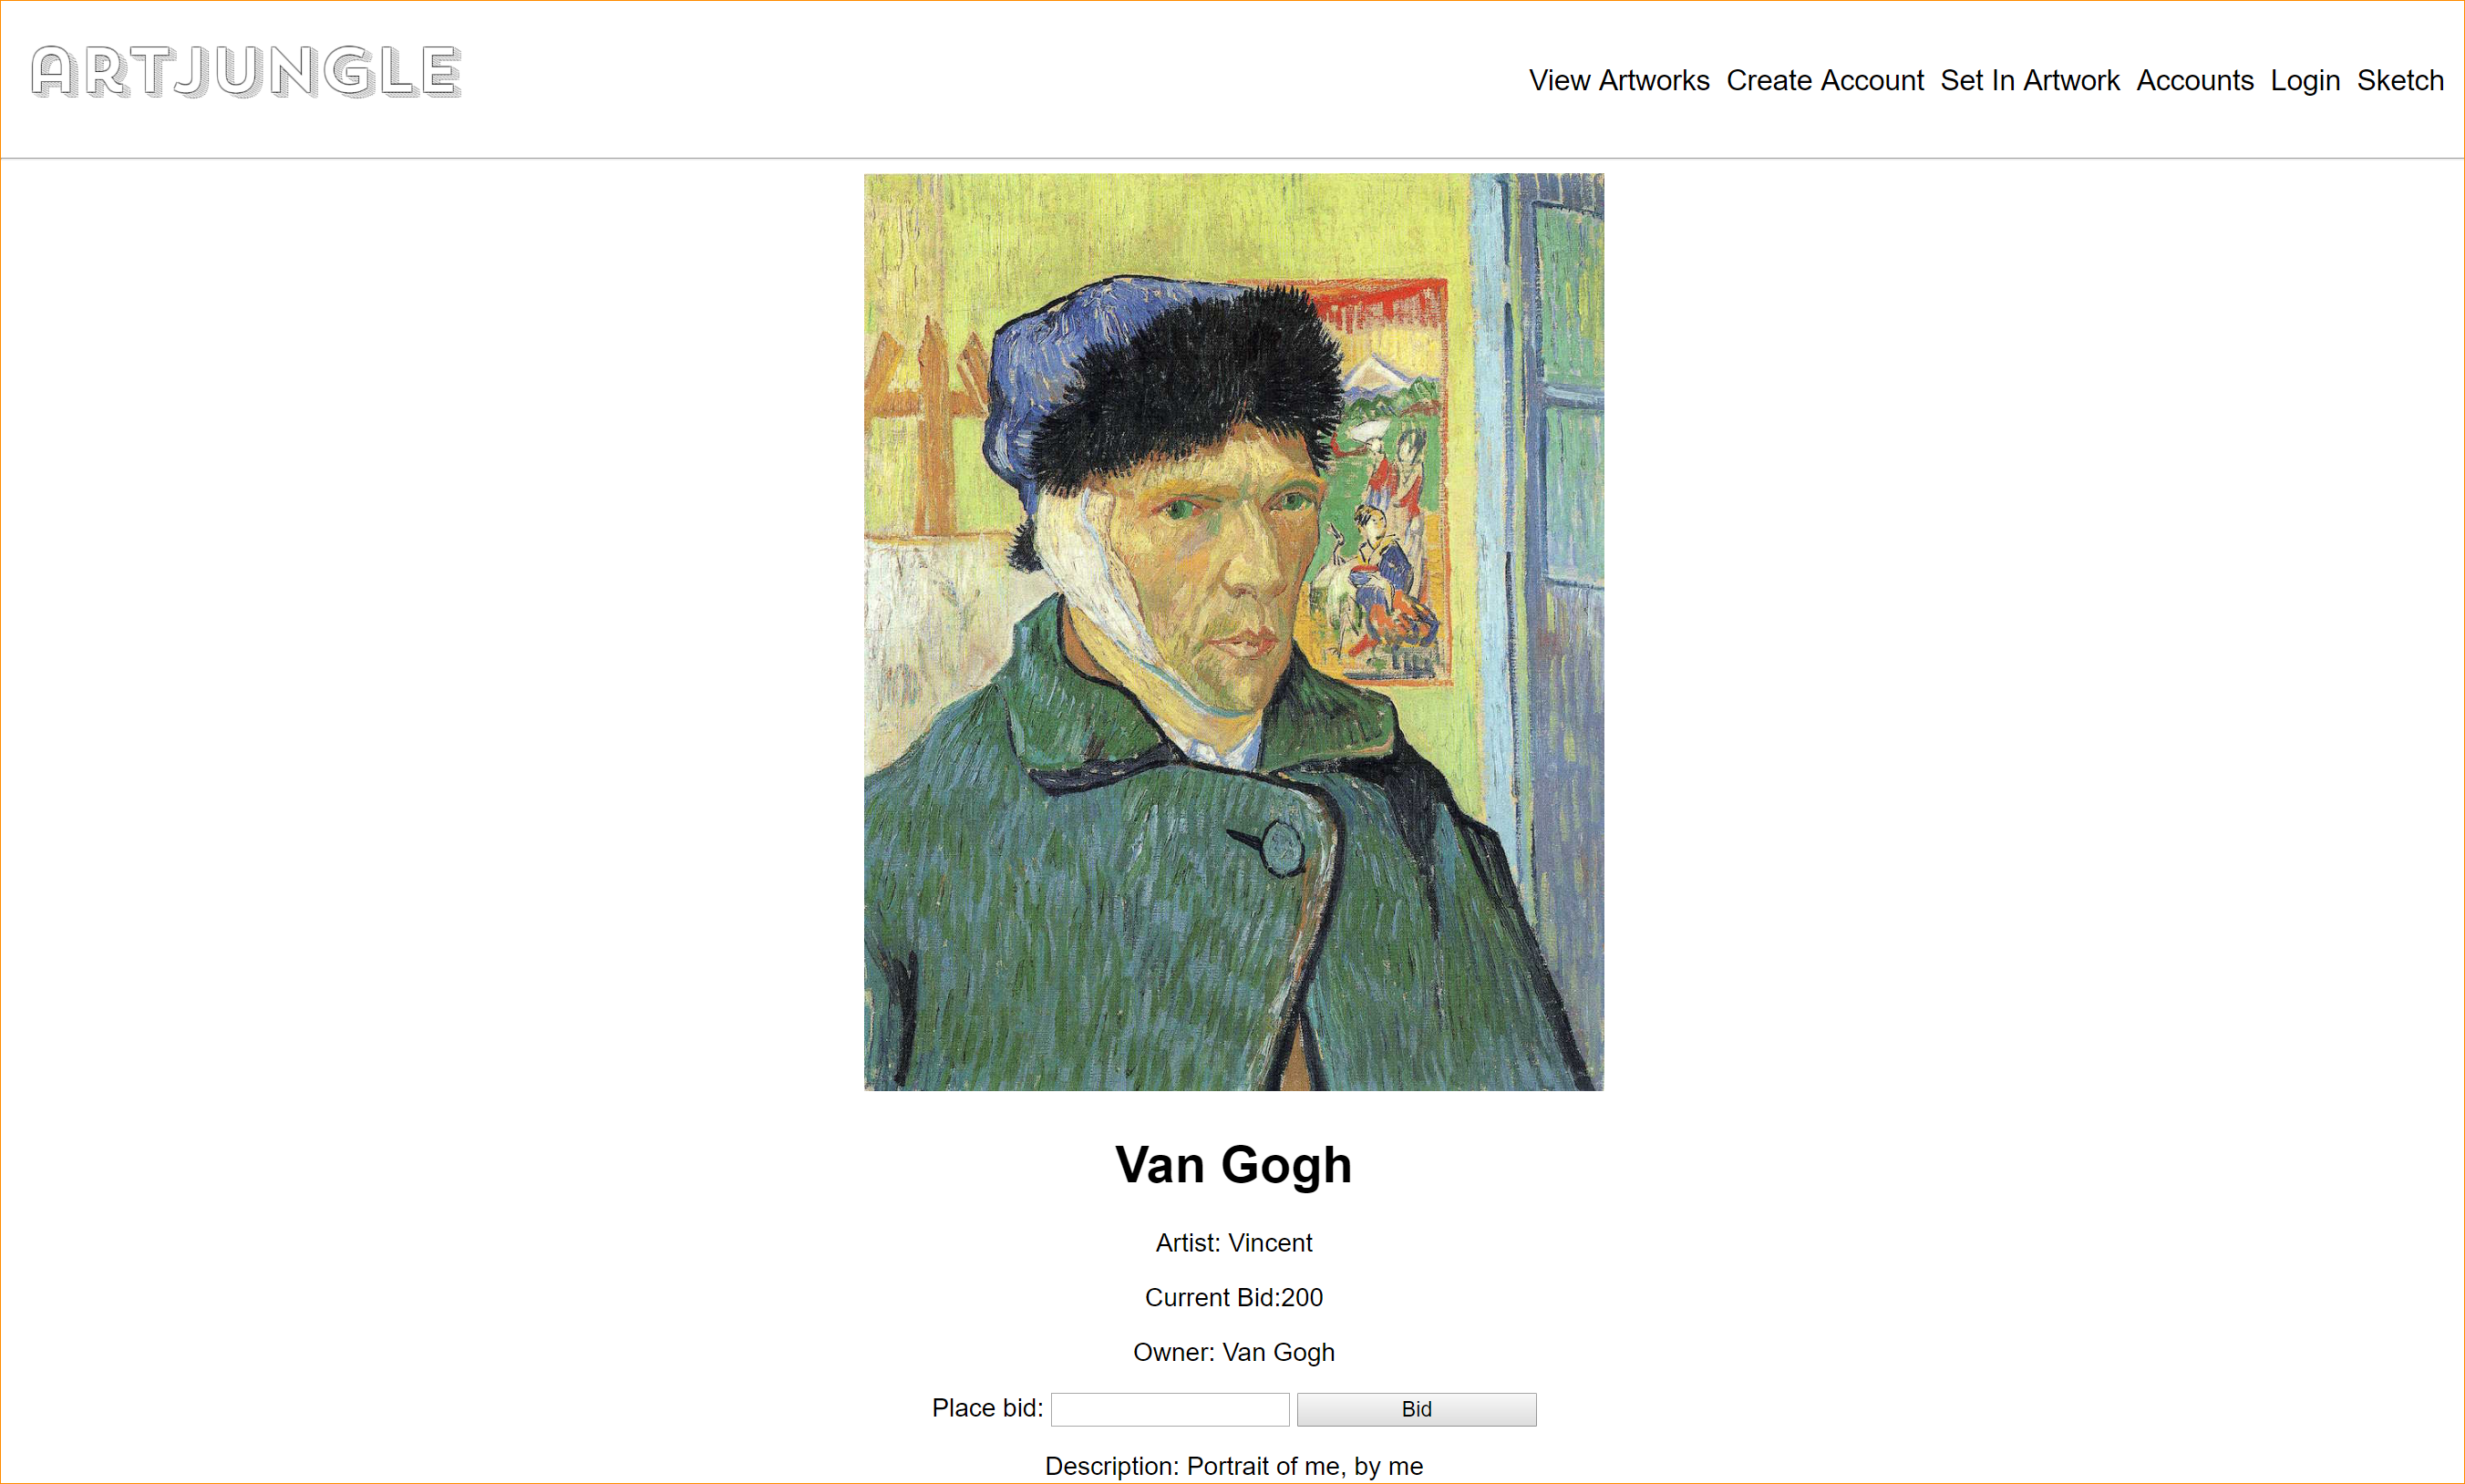
\includegraphics[scale=0.3]{figs/artwork.png}
  \caption{Details about an artwork}
\end{figure}

After clicking on an artwork, the user will see more details about the artwork, as shown in figure 6. The user will be able to bid on the artwork, and after a bid is made, the bid will be updated.  

\newpage
\begin{figure}[h!]
  \centering
  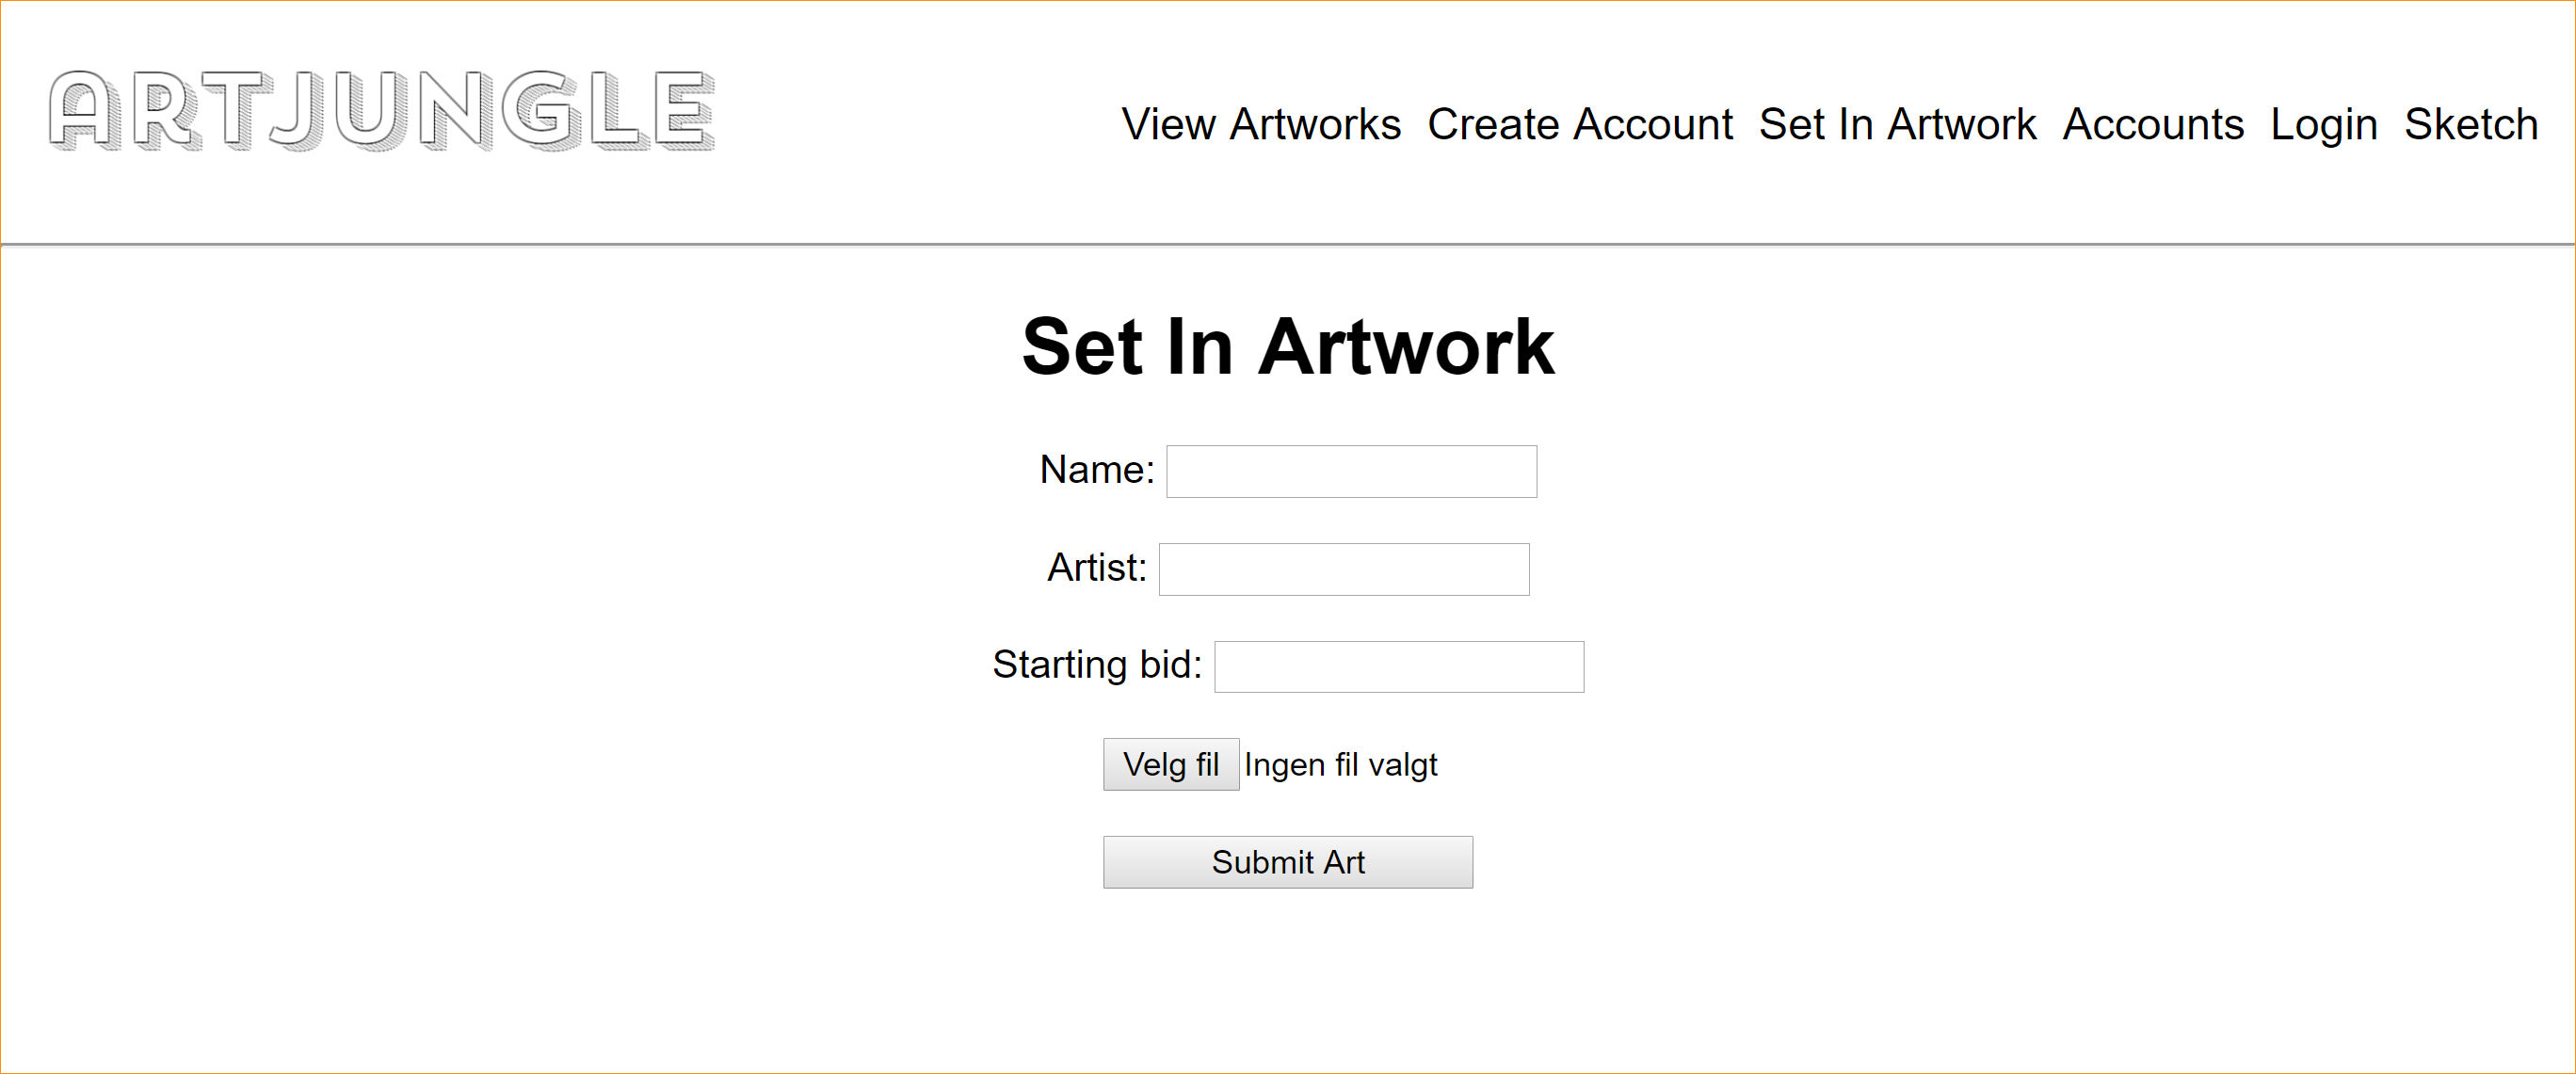
\includegraphics[scale=0.3]{figs/submitartwork.png}
  \caption{Submit an artwork}
\end{figure}

The user will be able to submit artworks by filling a form and adding an image of the artwork by clicking on "Set in Artwork", shown in figure 7. 

\begin{figure}[h!]
  \centering
  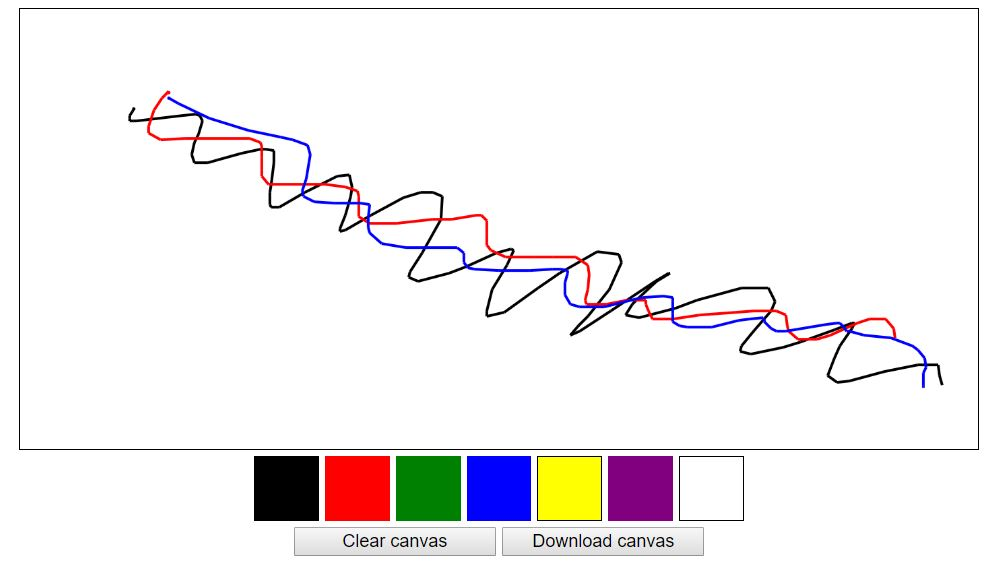
\includegraphics[scale=0.5]{figs/sketchApp.JPG}
  \caption{Details about an artwork}
\end{figure}

Lastly, the figure 8 shows that the user is able to draw on a canvas. The user can choose between multiple colors, clear the canvas or download the drawn image. With the module Socket.io, multiple users are able to draw on the same canvas at the same time. More details about this module will be mentioned later.

\subsection{The package.json}
The requirement of Node.js applications is the package.json file which contains several properties. Some of the crucial properties containing in the package.json file are name (name of the application), version, description (description of the application) and main (which points to the entry point of the application). The file also contains scripts (which will run when we need to perform repetitive tasks), author name, licence and dependencies. The properties summarize a representation of the Node.js application. 
\newline \newline
Listed below is our dependencies from \textbf{\textit{package.json}} used in our Node.js application.
\begin{minted}{json}
{
  ...
  "dependencies": {
    "bcrypt": "^1.0.3",
    "body-parser": "^1.18.3",
    "canvas2image": "^1.0.5",
    "ejs": "^2.6.1",
    "express": "^4.16.4",
    "express-fileupload": "^1.0.0",
    "formidable": "^1.2.1",
    "fs": "0.0.1-security",
    "mongodb": "^3.1.8",
    "mongoose": "^5.3.7",
    "morgan": "^1.9.1",
    "nodemon": "^1.18.6",
    "socket.io": "^2.1.1"
  }
}
\end{minted}
The dependencies are a requirement for the application. The modules must be installed to be able to run the prototype on another computer with Node.js, but can simply be installed with "npm install". 
\subsection{Architecture and implementation}
The architectural style is based on the MVC pattern. The Model-View-Controller Pattern defines the separation of the interconnected parts of our application. This is a commonly used framework of developing web applications. \cite{chrome:MVC}
\newline\newline
\textbf{Model}
\newline
Contains a representation of an object and also the logic to update the controller when data changes. The structure in this part covers Mongoose, which is a tool for MongoDB object modeling that works in an asynchronous environment. By using this tool we created a connection with MongoDB and defined our model through the Schema interface. Below we included code from the file \textbf{\textit{account.model.js}} to represent the structure of the account object.
\begin{minted}{JavaScript}
const AccountSchema = mongoose.Schema({
    name: String,
    phone: String,
    email: String,
    password: String,
    photo: String,
    bids: [{
        type: mongoose.Schema.Types.ObjectId,
        ref: 'Bid'
    }],
    artworks: [{
        type: mongoose.Schema.Types.ObjectId,
        ref: 'Artwork'
    }]
}, {
    timestamps: true
});
\end{minted}
Since MongoDB is a NoSQL database, there is not actual relation between the different entities in the model. But since we are using mongoose, we can just add the different entities like we did in the example above. This will save the id's of the relational entities, which can later be populated (see controller).
\\\\
\textbf{View}
\\
The view is the implementation and visualization of the data which the model includes. In this section we used Embedded JavaScript (EJS), which is a flexible template engine suited for Node.js. With EJS we can directly render pages dynamically with Express. Using EJS was simple, readable and convenient for the MVC structure. EJS makes it so that one can use functions such as .foreach() combined with the HTML code to avoid code repetition, as shown below from \textbf{\textit{view\_account.ejs}}.

\begin{minted}{HTML}
<% account.forEach(function(account) { %>
<div class="card">
    <a href="accounts/<%= account.id%>">
        <img src="<%= account.photo %>" style="width:100%; height:50%">
        <div class="container">
        
            <h3><%= account.name %></h3>
            <p>Phone: <%= account.phone %></p>
            <p>Email: <%= account.email %></p>
        </div>
    </a>
</div>
<% }); %>
\end{minted}
Here we get the account information in JSON-format from the backend, and use the .foreach() function to loop through each one and create the "cards" showing all the information for each account.
\\\\
\textbf{Controller}
\\
Separates the view and model while acting on both, by controlling the flow into model object when updating the view of the changed data. Here we created the REST API for our application. Here is an example from of the findAll() function from \textbf{\textit{account.controller.js}}.

\begin{minted}{JavaScript}
exports.findAll = (req, res) => {
    Account.find()
    .populate('bids')
    .populate('artworks')
    .then(account => {
        res.render('pages/view_accounts',{
            account:account
        })
    }).catch(err => {
        res.status(500).send({
            message: err.message || "Some error occurred while retrieving account."
        });
    });
};
\end{minted}
This is an event-handler for the REST API of our application. The function findAll() takes a request and response (req,res) as parameters, finds the requested accounts, populates the objects with data for the relations (see model), and sends the accounts back as a response (and renders the redirected page, this is ejs specific). If Account.find() returns an error, the error will be caught and an appropriate status code and message will be sent.
\\\\
We also attempted to create log-in functionality for the application, but we did not have the time to actually add functionalities like sessions and roles. We have added a password (which is hashed in the database) and log-in page to authenticate a user, but this has no actual purpose. 

\subsection{Development experience and Java EE comparison}
Setting up the the database and server for this prototype was a breeze compared to setting up the server and database in Eclipse when we created the Java EE application. It has also been much more stable for us, which has resulted in better flow in the development of the prototype. Also small things like restarting the GlassFish server in Eclipse was very slow, while the Express server in our prototype starts instantly (and automatically once we started using a package called nodemon), which made for a much better experience when developing the application.
\\\\
We also have some previous experience with JavaScript/TypeScript, and getting into the code in Node.js did not require much time and resource. We started with some simple tutorials for setting up the skeleton of the application with REST in an MVC architecture and developed from there. Harder tasks like asynchronous functions and callbacks also became manageable very quickly.
\\\\
Coding in Node.js and Java EE was actually pretty similar. Our biggest issues with developing the Java EE was not only code related, but rather the configurations and unstable server/database. We have a lot of experience with Java SE from before, so writing the code in Java EE was pretty simple (except new things like annotations and relations between entities) and the structure of the application was mostly straight forward. To compare the two here is a short codesnippet from the GET-request in the REST-API from each of the applications.
\\\\
Node.js:
\begin{minted}{JavaScript}
module.exports = (app) => {
  const artwork = require('../controllers/artwork.controller.js');
   app.get('/artworks', artwork.findAll);
   
   app.get('/artworks/:artworkId', artwork.findOne);
...
}
\end{minted}
Java EE:
\begin{minted}{Java}
...
@GET
@Path("/products")
@Produces({MediaType.APPLICATION_XML, MediaType.APPLICATION_JSON})
public Products getProducts() {
	return dao.getAllProducts();
}

@GET
@Path("/products/{id}")
public Response getProduct(@PathParam("id") String id) {
	Product product = dao.getProduct(id);
	if (product == null)
		throw new NotFoundException();
	return Response.ok(product).build();
}
...
\end{minted}
Both of these code snippets are methods/functions that basically do the same thing. They route a request to the business logic, where the data is retrieved from the database and is responded back. The difficulty of understanding the code here is pretty similar, but one can see that there is a big difference in the amount of code written, 5 lines for Node.js and 15 for Java EE (3x as many lines). This is mostly because of the method structure and annotations, whereas Node.js, which uses a listener (app), can handle the requests themselves in just one line each.
\\\\
Looking into a more quantitative comparison we can compare the total amount of lines of code.  Not taking into account such as dependencies, packages, tests and config files, we end up around 900 lines of code for Node.js project, and about 2300 lines for the Java EE. This makes sense since most of the code for Node.js is simpler, less structured and not as strongly typed, which makes it shorter. The Node.js prototype is also not as complex as the Java EE application. The Java EE application has multiple services, more entities and also a bit more functionality, so we have to take that into account. 
\\\\
If we look at the size on disk of the two projects though, we find something interesting. The Node.js project is taking up about 26.2 MB of space on disk (not counting .jpg files), whereas the entire Java EE project only takes up about 276 KB. This is mostly because of the nodemodules folder, that contains all the packages used, which takes up 26.1 MB of the 26.2 MB used. This leaves about 100KB of space for the rest of the files, which gives a more sensible code-to-diskspace ratio compared to the Java EE project. But one can see that because of Node.js projects have to save packages locally, it is not nearly as efficient as Java EE at using disc space.
\\\\
Our experience with developing a prototype using node.js has been good. Node.js was very simple to use, which one can tell by the progress we made with the prototype (compared to the Java EE application), and also at the amount of code written over this time period. Though it is lacking some robustness, security and structure compared to the Java EE application, it has been more stable, just as powerful and easier to make.
\section{Test Environment and Experimental Results}
\label{sec:experiments}

\subsection{Test bed}
Our test-bed will be our personal computers, whom all run the following configurations:
\begin{listing}
Web Server: Node.js HTTP-module (Express) \newline
Database: MongoDB Atlas\newline
Operative System: Windows 10 \newline
Browser: Google Chrome \newline
Programming Language: JavaScript
\end{listing}
\\\\
This test-bed is where we will do the development of the prototype. We will be testing the resilience of the prototype in a separate test-environment, in a virtual machine. More information about this in the next subsection.
\\\\
There were little to no problems with setting up the server and database connection for our test-bed. We started out with a local database, and migrated to a global MongoDB Atlas database once we had everything in place with the local database. We used some different software for actually creating the code for the prototype (Visual Studio Code and Atom), but this was just about personal preference and did not affect our development experience. 

\subsection{Test environment}
We wanted to run the application on a separate test-environment, to see if the prototype worked in another environment as well. We used VirtualBox to create the test-environment in a virtual machine with the following configurations:
\begin{listing}
Web Server: Node.js HTTP-module (Express) \newline
Database: MongoDB Atlas \newline
Operative System: Ubuntu Linux 64-bit \newline
Browser: Firefox \newline
Programming Language: JavaScript
\end{listing}
\\\\
Setting up the web application for our Linux Ubuntu test-environment was a simple task. All we had to do was install the right version of node (v8.12.0), install npm, clone the repository, use the "npm install" command in the folder containing the package.json file, and run the server script.
\\\\
Starting the server was no different than starting the server in windows, and the same went for connecting to the MongoDB database. We had some struggles with running the local database on other operating systems than windows, but ever since we migrated to a global MongoDB Atlas database, this has not been an issue for different environments. 
\\\\
Once everything was up and running, we could test our prototype in this new environment. The first thing to notice is that our test-environment uses Firefox, unlike our test-beds that run Google Chrome. This was not a problem for our application, as everything seemed to load properly, and looked as it should on the front-end side of the application. All functionality was working as intended, and even though the prototype was running on a virtual machine with limited resources, there was no sign of any drop in the performance of the application.

\subsection{Experiment overview}
Node.js is known for its power with real-time web applications, therefore our intention was to create some real-time functionality in our prototype and see how well it worked. For evaluating this experiment, we will look at how simple it was to create the desired functionality and look at the performance of the functionality under stress in the test-environment.
\\\\
Creating a real-time web application means that we will take advantage of Node.js concurrent programming abilities to develop some functionality that can be accessed and used by multiple users at the same time. Some examples of such functionality would be a live chat, live stream, etc. Since we went for an "art"-theme for our application, we decided it would be fun to create a live-drawing application (as shown in section 3.1), where multiple people can draw something at the same time online, save it, and put it up for auction.

\subsection{Experiment results}
Creating the drawing functionality did not require much implementation. As most things in Node.js, npm does most of the hard work for you. We used a package setting up the socket, where you installed the package called socket.io using npm, and then used some lines of code to deploy the socket as shown below. \cite{instructions:socketio}

\begin{minted}{JavaScript}

...
const io = require('socket.io')(server);
...
function onConnection(socket){
    socket.on('drawing', (data) => socket.broadcast.emit('drawing', data));
  }
  
io.on('connection', onConnection);
...
\end{minted}

Socket.io's GitHub page \cite{instructions:socketio} also has an example of a real-time drawing application, which was used to create our version of it in our application.
\\\\
For stress testing, we are trying to open up several instances of the sketch board at the same time on multiple computers (test environment and test bed computer, connected through IP address on LAN), and try to draw something at the same time, and see how it affects the performance. Our expectations of this is that it will behave normally up until about 50 windows each, where it might become very slow and unresponsive, or even freeze.
\\

\begin{table}[h]
\centering
\begin{tabular}{llrrrrrr}
  Windows open & Result
  \\ \hline \hline
1 & The default experience of the functionality \\ \hline 
25 & Smooth, no decrease in performance \\   
50 & Smooth, no decrease in performance \\
75 & Very slight lag at the start of drawing, smooth afterwards\\  
100 & Very clear lag at the start of drawing, smooth afterwards\\
125 & About 0.5 to 1 second delay before the drawing responds, less smooth overall\\  
\hline \hline
\end{tabular}
\caption{Stress test results}
\label{tab:results}
\end{table}

As we can see from our results in table 1, we started to notice some performance issue around 75 open windows. At 125 we stopped the test because now it starting to delay up to 1 second and the general experience started to be less smooth, and we were starting to close in on the limit of possible open windows for our VM at this point. Our application held up to our small stress-test very well, where it still performed quite well at 100+ open windows (it is entirely possible that having 100+ open windows makes the entire machine slow down, and the application itself was just as fast as with 2 windows). 

\section{Conclusions}

We have learned a lot in this project. We had heard about Node.js before, but didn't know what it did or how to use it. Throughout this project we have discovered a lot about the strengths and weaknesses of creating a web application in Node.js, and how the technology actually operates below the surface.
\\\\
Node.js lived up to its reputation of simplicity, hence our learning curve for creating the prototype has not been very steep. There were some bumps in the road, but it wouldn't take long before our issues were figured out. Things like good documentation, lots of information on the internet, a single language for both frontend and backend and the package handler contributed to the simplicity of this technology. 
\\\\
We also found that Node.js lived up to it's reputation of being powerful in many situations because of the event loop and Google's V8 engine. But this is only on a single thread, so given a problem that would require multiple threads (or thread resilience), then another technology like Java EE might be a better option.  
\\\\
After our hands-on experience of creating a web application in Node.js, we can clearly see why Node.js is one of the preferred option for creating these types of applications. Node.js popularity is also supported by the fact that JavaScript is one of, if not the most, popular programming language in the world, and it is continually growing in popularity. One aspect about JavaScript is that it also contributes to some of the drawbacks of Node.js. If qualities such as strongly typing, robustness and security is important, then Java EE would be a preferred option.
\\\\
Our experience with this technology was very good, even better than Java EE for creating this type of application. We found it to be very simple and powerful to use, even though it had it's drawbacks. We only compared it to one other technology in this report, but can come to the conclusion that Node.js would be, and often is, a very viable option compared to many other technologies for making web applications. 
\clearpage
\bibliographystyle{unsrtnat}
\bibliography{references}

\end{document}